\documentclass{article}
\usepackage{graphicx} % Required for inserting images
\usepackage{amsmath} % Required for some math notation
\usepackage{array} % allows for table notation
\usepackage{multirow} % allows for table notation
\usepackage[margin=1in]{geometry}

\title{Europa Induction Model}
\author{Neil Baker}
% \date{November 2026}

\begin{document}
\maketitle

%%%%%%%%%%%%%%%%%%%%%%%%%%%%%
%%%%%%%%%% SECTION %%%%%%%%%%
%%%%%%%%%%%%%%%%%%%%%%%%%%%%%
\section{Introduction}
Europa's material layers (out to in) consist of an icy crust, salty ocean, rocky mantle and iron core. ???

%%%%%%%%%%%%%%%%%%%%%%%%%%%%%
%%%%%%%%%% SECTION %%%%%%%%%%
%%%%%%%%%%%%%%%%%%%%%%%%%%%%%
\section{Model}
\begin{figure}[!b]
\begin{center}
\makebox[\textwidth][c]{
\noindent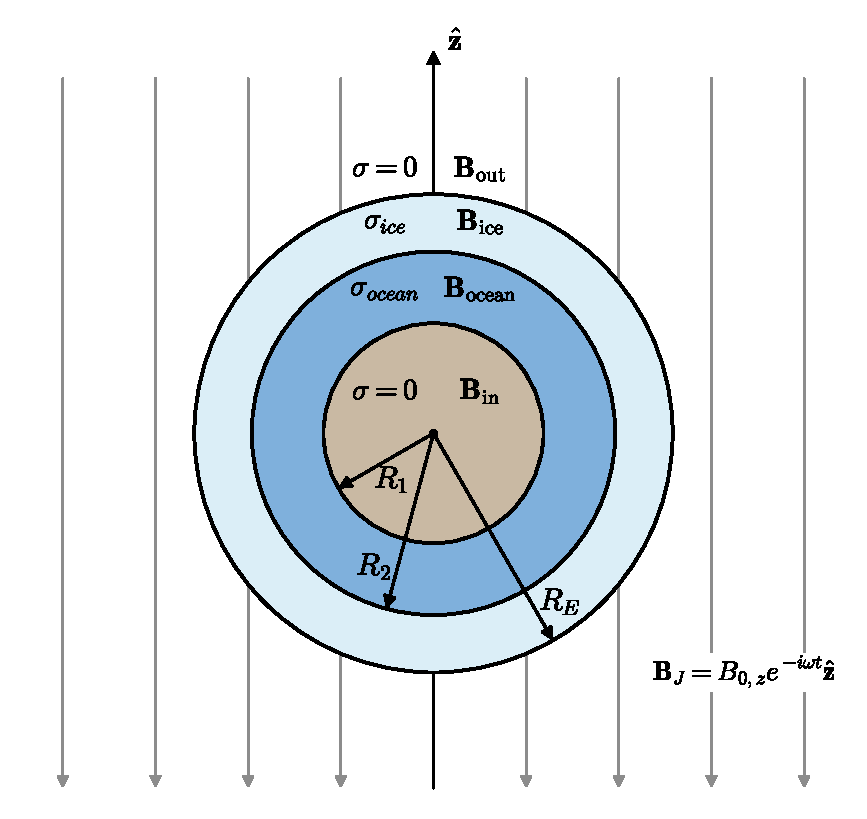
\includegraphics[width=0.5\textwidth]{Figures/shell_model.pdf}}
\caption{\scriptsize{\label{fig:shell_model}The shell model of Europa embedded in a one-dimensional, time-varying magnetic field $\mathbf{B}_J$. The $z$-direction points upwards and $\mathbf{B}_J$ (gray arrows) oscillates in this direction only. Europa's innermost volume (tan) has no conductivity and a radius $R_1$. The ocean (dark blue) extends from $R_1 < r < R_2$ and carries a conductivity $\sigma_{ocean}$. The ice shell (light blue) extends from $R_2 < r < R_E$ and carries a conductivity $\sigma_{ice}$.}}
\end{center}
\end{figure}
We use a spherical coordinate system $(r,\theta,\phi)$ with the origin at the center of the moon. We will assume that all of Europa's material layers are spherically symmetric. Europa's radius is denoted $R_E$. The interfaces between the mantle and the ocean, and the ocean and the crust occur at $r=R_1$ and $r=R_2$, respectively. We will \textit{only} consider the inductive response from these two layers; that is, we treat everything in the region $r<R_1$ as perfectly electrically insulating ($\sigma=0$). The ocean has conductivity $\sigma_{ocean}$, and the ice $\sigma_{ice}$. The conductivity profile is:
\begin{align}
    \sigma(r) &= \sigma_{ocean}[\Theta(r-R_1)-\Theta(r-R_2)] + \sigma_{ice}[\Theta(r-R_2)-\Theta(r-R_E)]
\end{align}
Where $\Theta$ is the Heaviside function. The ambient inducing Jovian magnetic field is the sum of a static field and an oscillating one, with variations in all three cartesian directions. We will omit the static part, which will only contribute add to the total field in the final solution and simply define the time-variable component, which is the inducing field.
\begin{align}
    \mathbf{B}_J(t) = \mathbf{B}_{0}e^{-i\omega t}
\end{align}
At any instant, $\mathbf{B}_J$ is uniform in space. We may split the inducing field up into its three cartesian components, which oscillate at the same synodic frequency, though they may be out of phase. Since Maxwell's equations and Ohm's law are linear and $\sigma(r)$ is spherically symmetric, the total induction response is equivalent to the sum of three individual signals in the $\mathbf{\hat{x}}$, $\mathbf{\hat{y}}$ and $\mathbf{\hat{z}}$ directions. By solving the problem with an inducing field along a single direction, the solutions in the other two will follow by rotation. We choose the $\mathbf{\hat{z}}$ direction to serve as the representative direction, where $z=r\cos(\theta)$ and $\mathbf{\hat{z}} = \cos(\theta)\mathbf{\hat{r}} - \sin(\theta)\boldsymbol{\hat{\theta}}$. In this way, the system has azimuthal symmetry.
\begin{align}
    \mathbf{B}_{J,z}(t) = B_{0,z}e^{-i\omega t}\mathbf{\hat{z}}
\end{align}

%%%%%%%%%%%%%%%%%%%%%%%%%%%%%
%%%%%%%%%% SECTION %%%%%%%%%%
%%%%%%%%%%%%%%%%%%%%%%%%%%%%%
\section{Fundamental Equations}
We will need the full set of Maxwell's equations, minus the displacement current, plus Ohm's law. We utilize the $\mathbf{E}$ and $\mathbf{B}$ fields rather than the $\mathbf{D}$ and $\mathbf{H}$ fields because ???.
\begin{align}
    \nabla\cdot\mathbf{E} &= \frac{\rho_c}{\epsilon_0} \label{Gauss} \\
    \nabla\cdot\mathbf{B} &= 0 \label{DivB} \\
    \nabla\times\mathbf{E} &= -\frac{\partial\mathbf{B}}{\partial t} \label{Faraday} \\
    \nabla\times\mathbf{B} &= \mu_0\mathbf{j} \label{Ampere} \\
    \mathbf{j} &= \sigma\mathbf{E} \label{Ohm}
\end{align}
We do not consider the displacement current, $\partial_t\mathbf{E}/c^2$, where $c$ is the speed of light. The Jovian field has a period of around 11 hours. On these time scales, $\partial_t\mathbf{E}$ is small compared to $c^2$, and relativistic corrections can be readily neglected.

%%%%%%%%%%%%%%%%%%%%%%%%%%%%%
%%%%%%%%%% SECTION %%%%%%%%%%
%%%%%%%%%%%%%%%%%%%%%%%%%%%%%
\section{Boundary Conditions}
A correct description of the magnetic field boundary conditions is crucial to describe it everywhere in space.  

\end{document}
